\documentclass[12pt,a4paper]{article}
\usepackage{graphicx}
\usepackage{wrapfig}

\title{Praktikum Physik - Fallzeit}
\author{Simon Marti, Patricia Schwab, Mirco Kocher}
\date{24.02.2012}
\newcommand{\h}{1.044 }

\begin{document}
\maketitle

%%
% Ziel
%%
\section*{Ziel}
Messung der Fallzeit einer Metallscheibe und Berechnung der Fallbeschleunigung.

%%
% Motivation
%%
\section*{Motivation}
Die Messung der Fallzeit von Hand mit einer Stoppuhr eignet sich sehr gut um den Umgang mit Messfehlern kennenzulernen. 

%%
% Theorie
%%
\section*{Theorie}
Die Fallzeit eines Objektes aus H\"ohe $h$ ist, unter Vernachl\"assigung des Luftwiederstandes, durch folgende Formel gegeben:
\[ h = \frac{1}{2}gt^2 \]
Die Fallbeschleunigung $g$ h\"angt von der geographischen Breite $\Phi$ sowie der H\"ohe \"uber dem Meeresspiegel $H$ ab.
\[ g = 9.80616 - 0.25928\cdot \cos (2\Phi ) + 0.000069\cdot \cos^2(\Phi ) - 3.086\cdot 10^{-7}H \]
F\"ur Bern ($\Phi = 47^{\circ}$ und $H = 550$m) ergibt dies einen theoretischen Wert von
\[ g = 9.80783 \]

%%
% Experiment
%%
\pagebreak
\section*{Experiment}
\subsection*{Aufbau und Ablauf}
\begin{wrapfigure}{r}{8cm}
\vspace{-50pt}
\centering
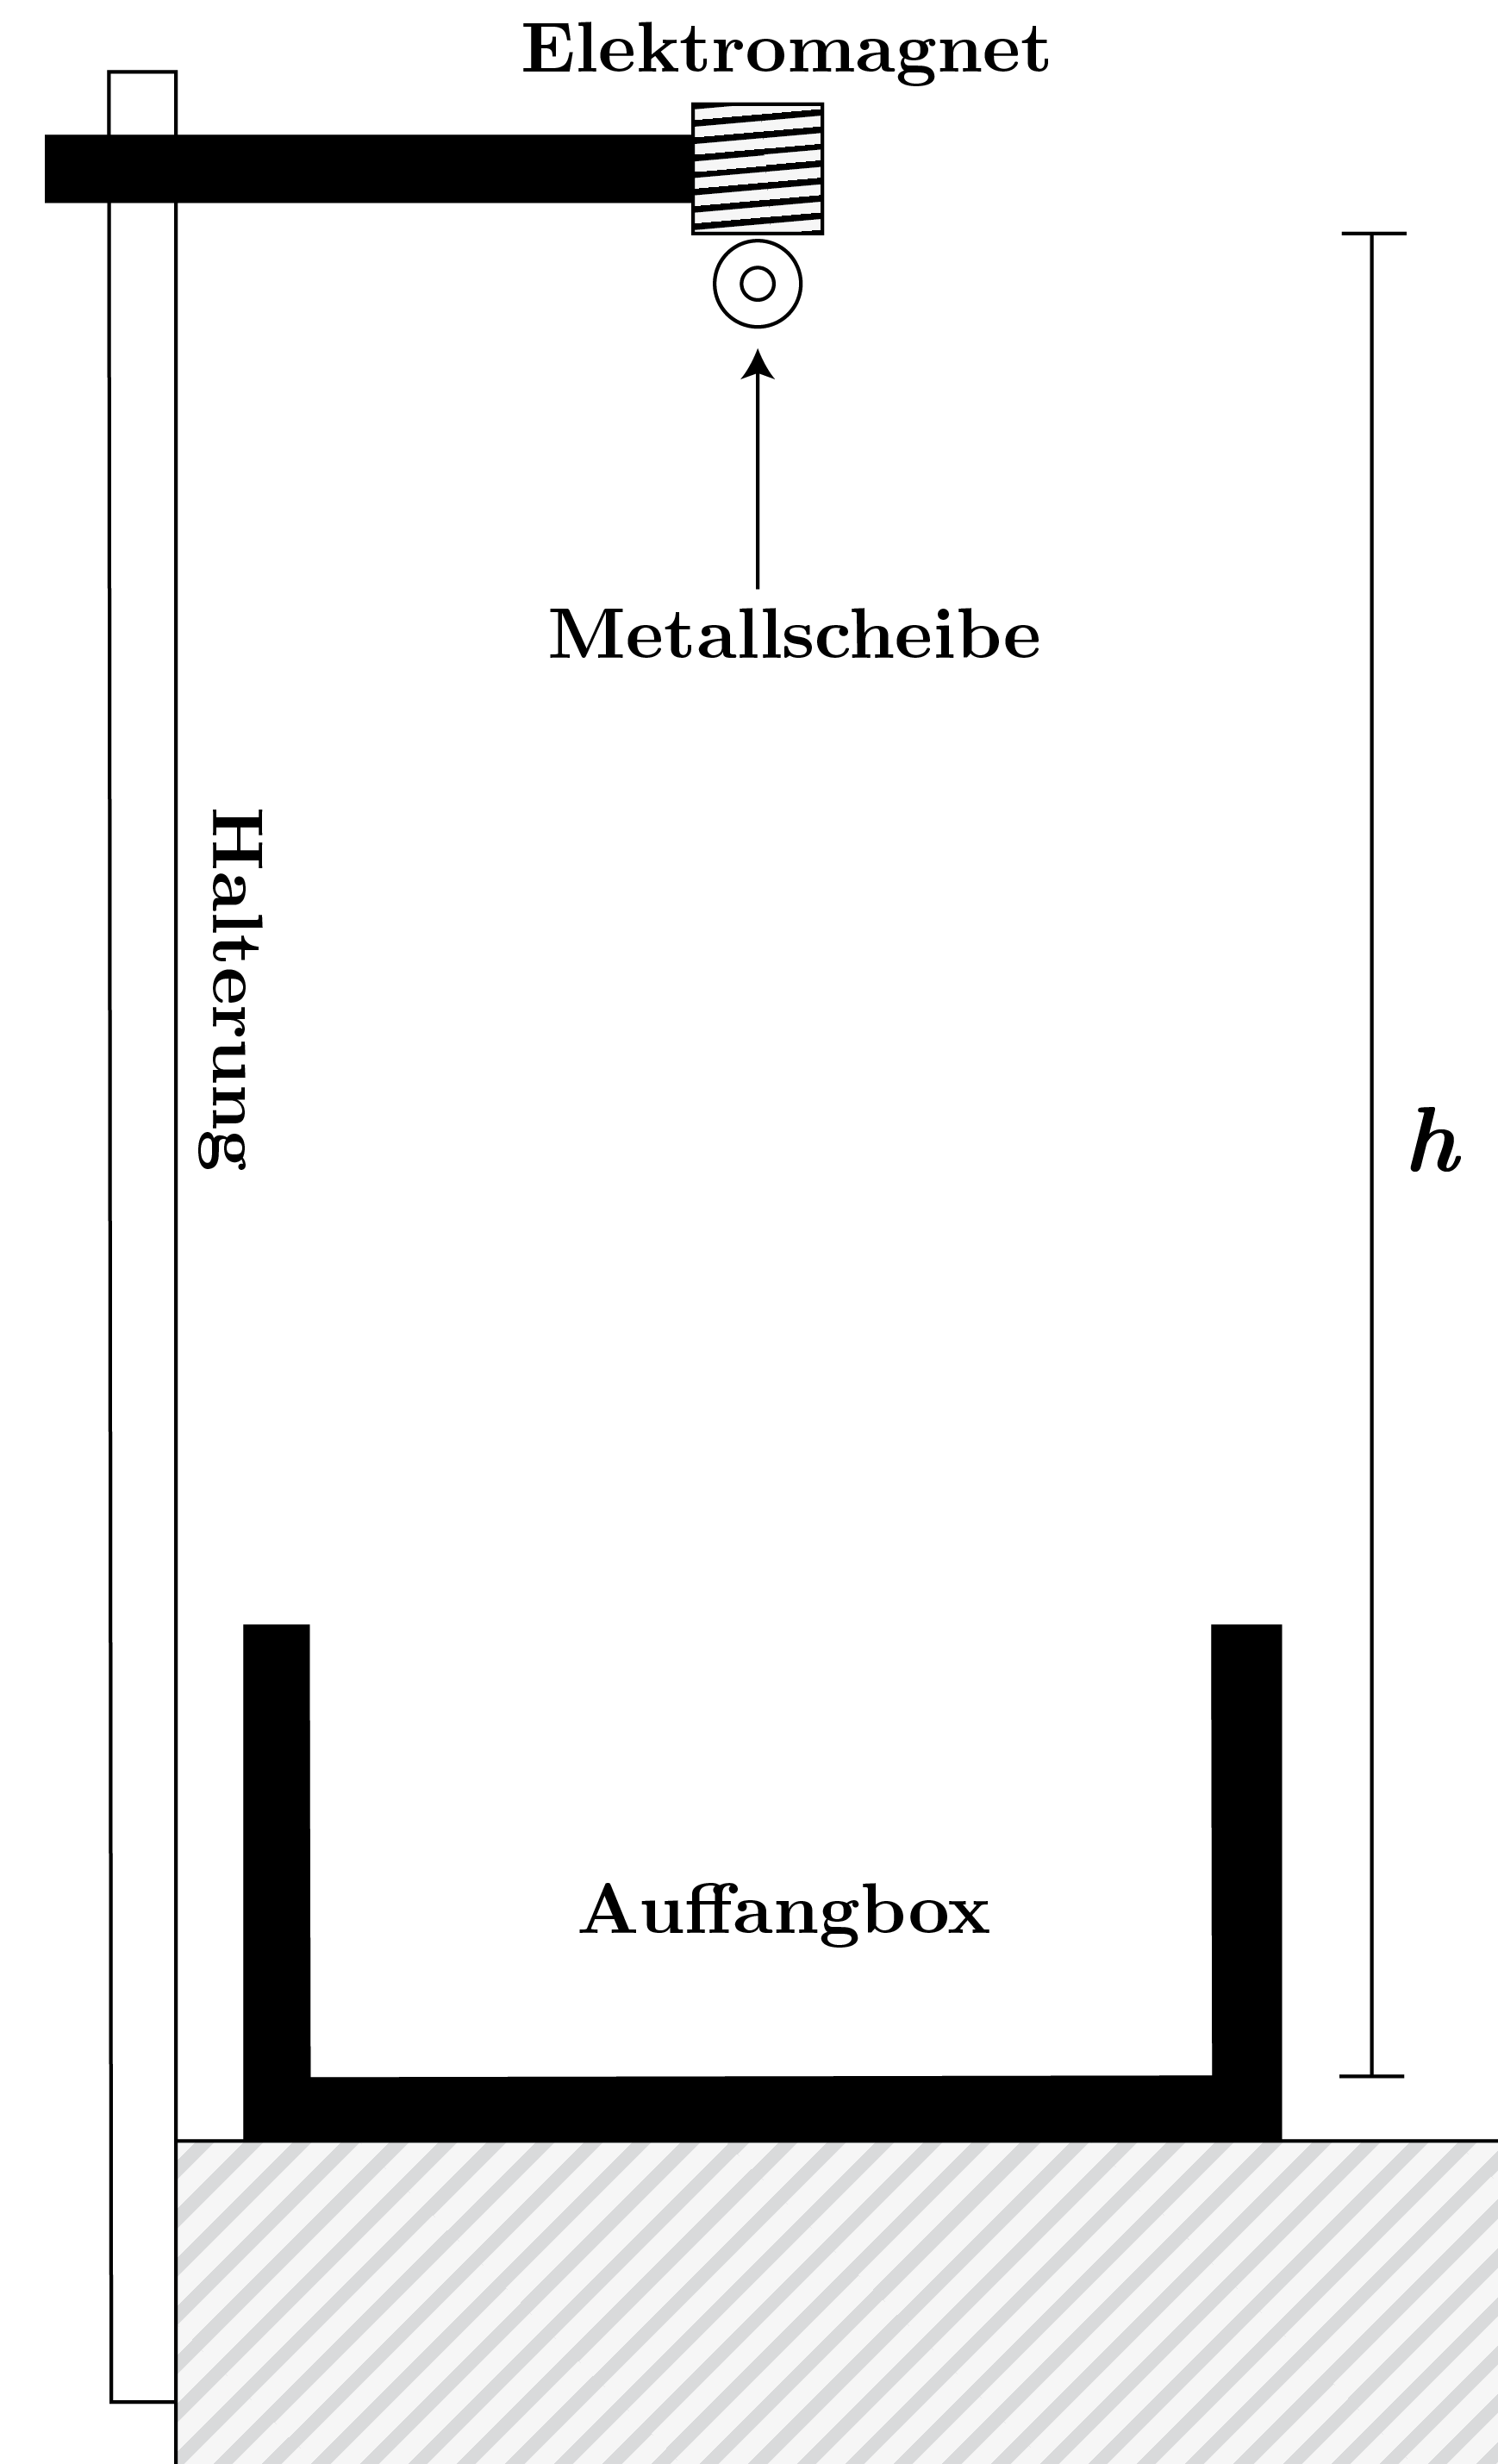
\includegraphics[width=6cm]{experiment.png}
\end{wrapfigure}
Ein Elektromagnet ist an einem Metallgestell \"uber einer Auffangbox befestigt und h\"alt eine Metallscheibe fest. Der Abstand des Magneten zum Boden der Auffangbox bezeichnen wir als $h$. Der Elektromagnet ist mit einem Taster verbunden, der den Stromzufluss zu diesem unterbricht worauf die Metallscheibe frei in die Auffangbox f\"allt. Die Fallzeit der Scheibe wird mit einer Stopp\-uhr manuell gemessen.

%%
% Rohdaten
%%
\subsection*{Rohdaten}
\subsubsection*{Zeitmessung}
\begin{tabular}{|r|l|r|l|r|l|r|l|r|l|r|l|}
\hline
\#&$t$&\#&$t$&\#&$t$&\#&$t$&\#&$t$&\#&$t$\\
\hline
1&0.38s&18&0.45s&35&0.41s&52&0.43s&69&0.45s&86&0.45s\\
2&0.45s&19&0.41s&36&0.39s&53&0.43s&70&0.43s&87&0.40s\\
3&0.48s&20&0.44s&37&0.41s&54&0.41s&71&0.41s&88&0.43s\\
4&0.38s&21&0.43s&38&0.43s&55&0.40s&72&0.41s&89&0.44s\\
5&0.45s&22&0.41s&39&0.44s&56&0.48s&73&0.45s&90&0.45s\\
6&0.50s&23&0.48s&40&0.42s&57&0.43s&74&0.42s&91&0.43s\\
7&0.41s&24&0.41s&41&0.41s&58&0.38s&75&0.45s&92&0.41s\\
8&0.43s&25&0.44s&42&0.45s&59&0.40s&76&0.41s&93&0.47s\\
9&0.41s&26&0.44s&43&0.42s&60&0.44s&77&0.44s&94&0.45s\\
10&0.41s&27&0.43s&44&0.46s&61&0.41s&78&0.44s&95&0.45s\\
11&0.41s&28&0.44s&45&0.44s&62&0.45s&79&0.45s&96&0.44s\\
12&0.41s&29&0.42s&46&0.41s&63&0.45s&80&0.41s&97&0.42s\\
13&0.45s&30&0.42s&47&0.44s&64&0.44s&81&0.45s&98&0.40s\\
14&0.45s&31&0.46s&48&0.41s&65&0.44s&82&0.43s&99&0.42s\\
15&0.46s&32&0.42s&49&0.41s&66&0.43s&83&0.41s&100&0.41s\\
16&0.43s&33&0.47s&50&0.37s&67&0.43s&84&0.45s&&\\
17&0.41s&34&0.45s&51&0.37s&68&0.41s&85&0.48s&&\\
\hline
\end{tabular}

\subsubsection*{H\"ohenmessung}
Die H\"ohe $h$ wurde auf ($1.044 \pm 0.005$) m gemessen.

%%
% Kontrollrechnung
%%
\subsection*{Kontrollrechnung}
Aus der gemessenen H\"ohe $h$ folgt eine theoretische Fallzeit von
\[ t = \sqrt{\frac{2h}{g}} = \sqrt{\frac{2\cdot 1.044}{9.808}} = 0.461\mbox{s} \]
Dieser Wert liegt innerhalb der ersten drei Messwerten.

%%
% Auswertung
%%
\subsection*{Auswertung}
\subsubsection*{Statistische Daten}'
\begin{tabular}{ll}
Anzahl Messungen:&100\\
Durchschnitt $\overline{t}$:&0.430s\\
Standardabweichung $s_t$:&0.025s\\
Fehler des Mittelwerts $s_{\overline{t}}$:&0.0025s\\	
\end{tabular}

\subsubsection*{Verteilung der Messwerte}
Der markierte Bereich entspricht der Standardabweichung.

\begin{center}
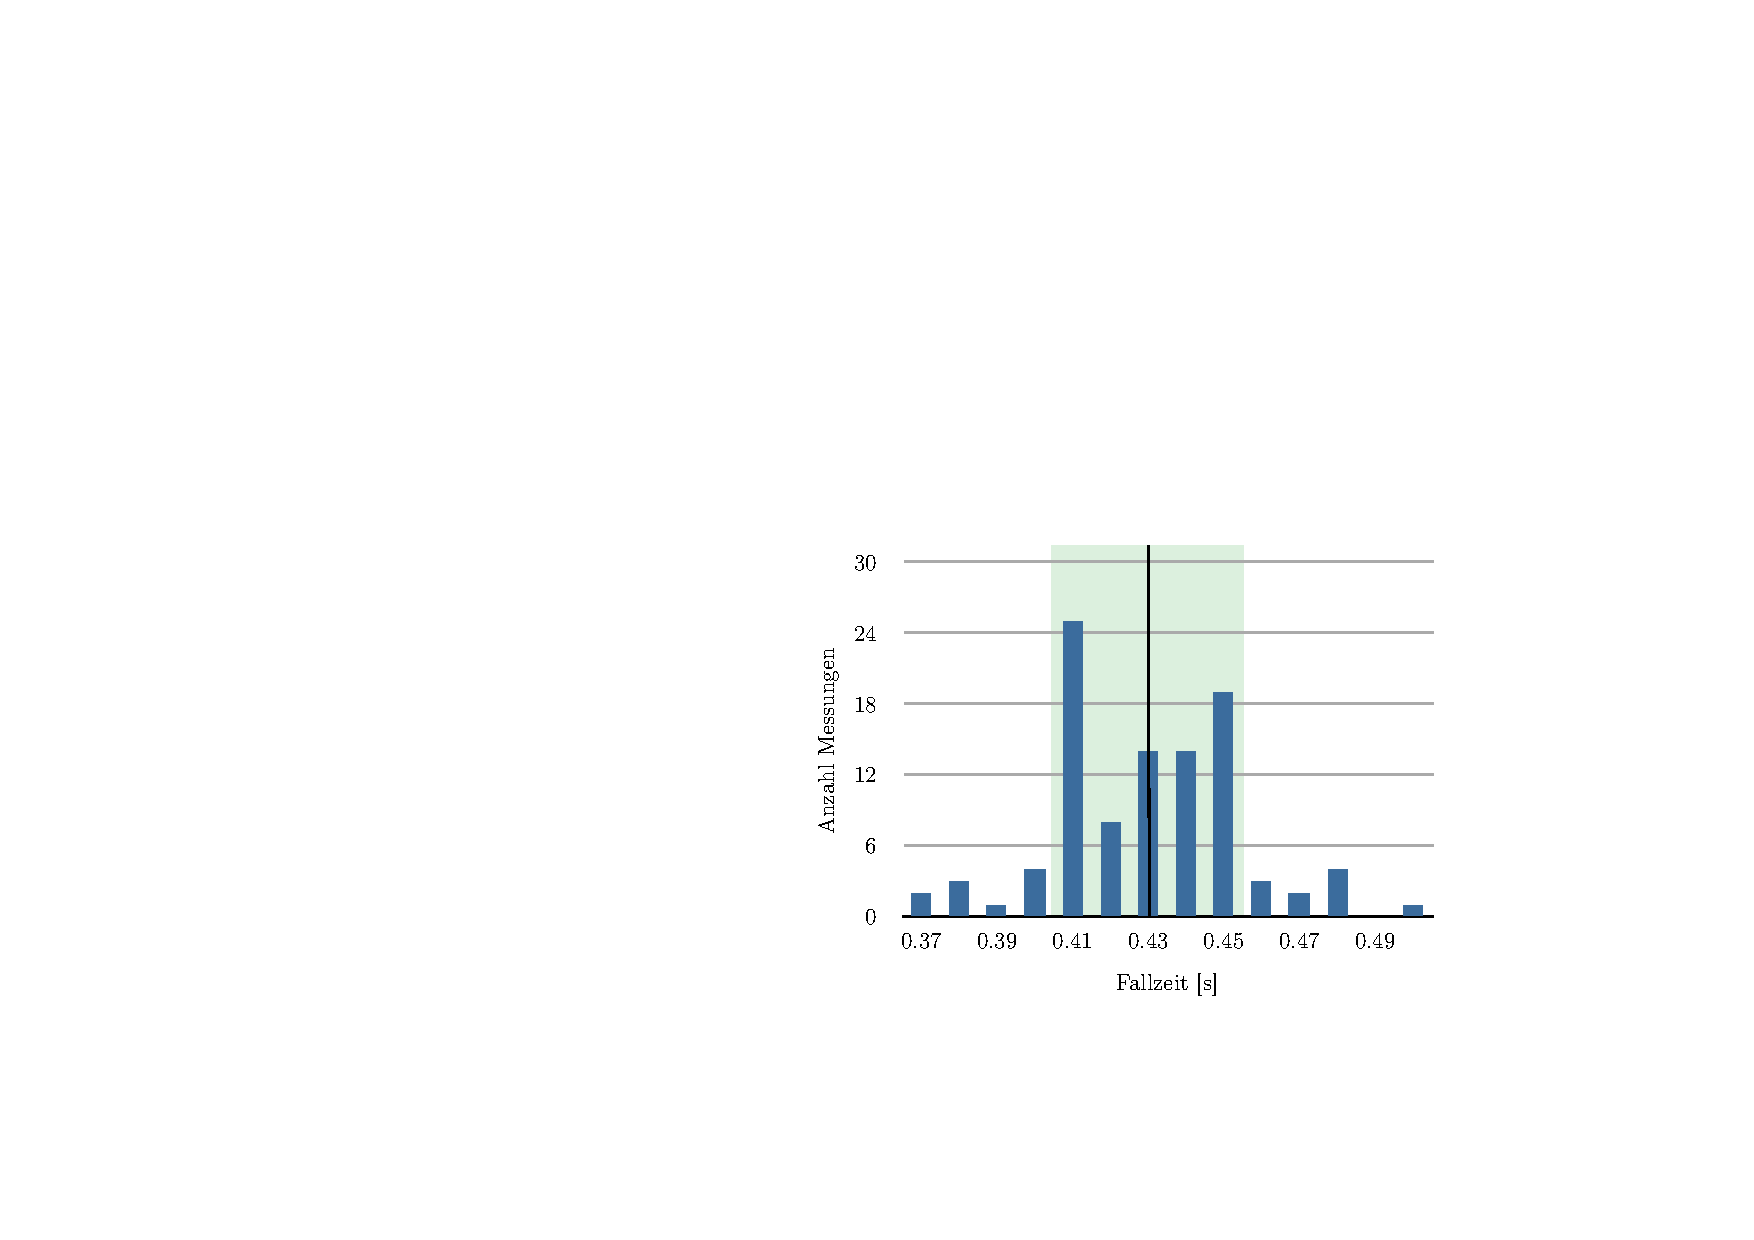
\includegraphics[width=12cm]{histogram.pdf}
\end{center}

\subsubsection*{Fehler der Fallbeschleunigung}
Ausgehend von der Formel aus dem Theorieteil kann die Fallbeschleunigung wie folgt berechnet werden:
\[ g = \frac{2h}{t^2} \]
Da $g$ sowohl von $h$ als auch von $t$ abh\"angt gilt:
\[ s_g^2 = \left( \frac{\partial g}{\partial t}\right)^2 s_t^2 + \left( \frac{\partial g}{\partial h}\right)^2 s_{h}^2 \]
\[ \frac{\partial g}{\partial t} = \frac{-4h}{t^3} \hspace{30pt} \frac{\partial g}{\partial h} = \frac{2}{t^2} \]
\[ s_g^2 = \left| \frac{16hs_t^2}{t^6}\right| + \left| \frac{4s_h^2}{t^4}\right| \Rightarrow s_g = 0.140 \mbox{ms}^{-2} \]

\subsubsection*{Zusammenfassung}
\begin{tabular}{rcl}
t & = & (0.430 $\pm$ 0.0025) s\\
h & = & (\h $\pm$ 0.005) m\\
g & = & (11.319 $\pm$ 0.140) ms${}^{-2}$\\
\end{tabular}

\section*{Diskussion}
Die Experimentell ermittelte Fallbeschleunigung weicht relativ stark (\"uber 15\%) vom Tabellenwert ab was vermutlich gr\"osstenteils auf die ungenaue Messung der Zeit mit einer Stoppuhr zur\"uckzuf\"uhren ist. Die gemessenen Werte weisen zwar nur einen geringen statistischen Fehler auf, doch es scheint ein viel gr\"osserer systematischer Fehler vorzuliegen der dadurch hervorgerufen wurde, dass die Zeit konsequent zu kurz gestoppt wurde.

\end{document}